\documentclass{article}
\usepackage{amsmath, amssymb, amsthm}
\usepackage{graphicx}
\usepackage[colorlinks=true, linkcolor=blue, citecolor=black, backref=page]{hyperref}
\usepackage{lscape}
\usepackage{placeins}
\usepackage{listings}
\usepackage{xcolor}
\usepackage{float}

% Define custom colors
\definecolor{dkgreen}{rgb}{0,0.6,0}
\definecolor{gray}{rgb}{0.5,0.5,0.5}
\definecolor{mauve}{rgb}{0.58,0,0.82}

% Configure lstlisting settings for Python
\lstset{
  frame=tb,                      % Draw a frame at the top and bottom of the code block
  language=Python,               % Set the language to Python
  aboveskip=3mm,                 % Add space above the code block
  belowskip=3mm,                 % Add space below the code block
  showstringspaces=false,        % Do not display string spaces with special underlines
  columns=flexible,              % Allow flexible column spacing
  basicstyle={\small\ttfamily},  % Set the font style and size for code
  numbers=left,                  % Display line numbers on the left
  numberstyle=\tiny\color{gray}, % Style for line numbers
  keywordstyle=\color{blue},     % Style for keywords
  commentstyle=\color{dkgreen},  % Style for comments
  stringstyle=\color{mauve},     % Style for strings
  breaklines=true,               % Allow long lines to break
  breakatwhitespace=true,        % Break lines at whitespace if possible
  tabsize=4                      % Set tab size to 4 spaces
}

\begin{document}

\title{NLO Assignment 2}
\author{}
\date{\today}
\maketitle

\section{Find all the KKT points.}\label{sec:a}



\subsection{Convexity of the Objective Function}
The given objective function is:
\begin{equation}
f(x_1, x_2) = \frac{1}{2}x_1^2 - x_2^2.
\end{equation}
To determine convexity, we compute its Hessian matrix:
\begin{equation}
H = \begin{bmatrix} 
\frac{\partial^2 f}{\partial x_1^2} & \frac{\partial^2 f}{\partial x_1 \partial x_2} \\ 
\frac{\partial^2 f}{\partial x_2 \partial x_1} & \frac{\partial^2 f}{\partial x_2^2} 
\end{bmatrix}
=
\begin{bmatrix} 
1 & 0 \\ 
0 & -2 
\end{bmatrix}.
\end{equation}

For $f(x_1, x_2)$ to be convex, the Hessian must be positive semi-definite, meaning all its eigenvalues must be non-negative. The eigenvalues of $H$ are:
\begin{equation}
\lambda_1 = 1, \quad \lambda_2 = -2.
\end{equation}
Since one eigenvalue is negative, the Hessian is not positive semi-definite. Therefore, \textbf{the objective function is not convex}.

\subsection{Nature of the Constraint}
The given constraint is:
\begin{equation}
x_1^2 + x_2^2 \leq 1.
\end{equation}
Since this constraint contains quadratic terms, it is \textbf{not linear}. However, it represents a convex set (a disk in $\mathbb{R}^2$), since the function $g(x) = x_1^2 + x_2^2 - 1$ is convex.




The Lagrangian function for this problem is:
\begin{equation}
L(x_1, x_2, \lambda) = \frac{1}{2}x_1^2 - x_2^2 + \lambda (x_1^2 + x_2^2 - 1),
\end{equation}
where $\lambda \geq 0$ is the Lagrange multiplier.

\newpage

\textbf{The Karush-Kuhn-Tucker (KKT) conditions are as follows:}

\textbf{Stationarity:}
\begin{equation}
\nabla_{x_1} L = \frac{\partial L}{\partial x_1} = x_1 + 2\lambda x_1 = 0
\end{equation}
\begin{equation}
\nabla_{x_2} L = \frac{\partial L}{\partial x_2} = -2x_2 + 2\lambda x_2 = 0
\end{equation}

\textbf{Primal Feasibility:}
\begin{equation}
x_1^2 + x_2^2 \leq 1
\end{equation}

\textbf{Dual Feasibility:}
\begin{equation}
\lambda \geq 0
\end{equation}

\textbf{Complementary Slackness:}
\begin{equation}
\lambda g(x_1, x_2) = \lambda(x_1^2 + x_2^2 - 1) = 0
\end{equation}

\subsection{Finding the KKT Points}

\textbf{Case 1: $\lambda = 0$ (Inactive Constraint)}

\begin{equation}
\text{Stationarity: } 
\begin{cases}
x_1(1 + 2\lambda) = 0 \\
x_2(-2 + 2\lambda) = 0
\end{cases}
\end{equation}

\begin{equation}
\text{With } \lambda = 0:
\begin{cases}
x_1(1 + 2(0)) = 0 \implies x_1 = 0 \\
x_2(-2 + 2(0)) = 0 \implies x_2 = 0
\end{cases}
\end{equation}

\begin{equation}
\text{Since } 0^2 + 0^2 \leq 1, (0, 0, 0) \text{ is a KKT point.}
\end{equation}

\textbf{Case 2: $\lambda > 0$ (Active Constraint)}

\begin{equation}
\text{Complementary Slackness: } x_1^2 + x_2^2 = 1
\end{equation}

\begin{equation}
\text{Stationarity: } 
\begin{cases}
x_1(1 + 2\lambda) = 0 \\
x_2(-2 + 2\lambda) = 0
\end{cases}
\end{equation}

\begin{equation}
\text{If } x_1 \neq 0, \text{ then } 1 + 2\lambda = 0 \implies \lambda = -\frac{1}{2}, \text{ violating } \lambda \geq 0.
\end{equation}

\begin{equation}
\text{Thus, } x_1 = 0.
\end{equation}

\begin{equation}
\text{Also, } x_2(-2 + 2\lambda) = 0.
\end{equation}

\begin{equation}
\text{If } x_2 = 0, \text{ then } x_1^2 + x_2^2 = 0, \text{ contradicting } x_1^2 + x_2^2 = 1.
\end{equation}

\begin{equation}
\text{Therefore, } -2 + 2\lambda = 0 \implies \lambda = 1.
\end{equation}

\begin{equation}
\text{With } x_1 = 0, x_2^2 = 1, \text{ so } x_2 = \pm 1.
\end{equation}

\begin{equation}
\text{Thus, } (0, 1, 1) \text{ and } (0, -1, 1) \text{ are KKT points.}
\end{equation}

\begin{equation}
f(x,y) = \begin{cases}
\frac{1}{2}x^2 - y^2, & \text{if } (x,y) = (0,0) \\
\frac{1}{2}x^2 - y^2, & \text{if } (x,y) = (0,1) \\
\frac{1}{2}x^2 - y^2, & \text{if } (x,y) = (0,-1)
\end{cases}
\end{equation}

\begin{equation}
\text{Values of } f(x,y):
\begin{cases}
f(0,0) = \frac{1}{2}(0)^2 - (0)^2 = 0 \\
f(0,1) = \frac{1}{2}(0)^2 - (1)^2 = -1 \\
f(0,-1) = \frac{1}{2}(0)^2 - (-1)^2 = -1
\end{cases}
\end{equation}

Evaluating the objective function, $\frac{1}{2}x_1^2 - x_2^2$, at points $(0,1)$ and $(0,-1)$, the function attains a value of $-1$, indicating we have achieved minimization. But, at $(0,0)$, the function value is $0$, which is greater than $-1$, thereby making $(0,0)$ a saddle point rather than a minimum. Therefore, the function is minimized at $(0,1)$ and $(0,-1)$ with a value of $-1$, and $(0,0)$ is a saddle point. For more clarity one can look at the graph at the end of the solutions in the appendix--section \ref{sec:d} to have a pictorial understanding. In addition, more analysis towards justifying this is carried out in $1(c)$--section \ref{sec:c}.

\subsection{Conclusion}

The KKT points are:
\[
(0,0,0), \quad (0,1,1), \quad (0,-1,1).
\]
Among these, $(0,1)$ and $(0,-1)$ are the global minimizers, achieving the lowest function value of $-1$. The point $(0,0)$ is a saddle point.

\newpage
\section{State the Slater Constraint Qualification(SCQ) and show that it is satisfied}\label{sec:b}


For a convex optimization problem which takes the form:

\begin{align*}
\text{Minimize: } & f_0(x) \\
\text{Subject to: } & f_i(x) \leq 0, \quad i = 1, \ldots, m
\end{align*}

SCQ holds if:

\begin{enumerate}
    \item All of $f_i(x)$ are convex in  nature.
    \item There exist an $x$ such a way that $f_i(x) < 0$ for all $i = 1, \ldots, m$.
\end{enumerate}

\textbf{Verification:}

\begin{enumerate}
    \item \textbf{Convexity:}
        \begin{itemize}
            \item $f_1(x_1, x_2) = x_1^2 + x_2^2$ is a convex function.
            \item $f_0(x_1, x_2) = \frac{1}{2}x_1^2 - x_2^2$ is \textbf{not} a convex function.
        \end{itemize}
    \item \textbf{Strict Feasibility:}
        \begin{itemize}
            \item We need to find $(x_1, x_2)$ such that $f_1(x_1, x_2) < 1$.
            \item Let $(x_1, x_2) = (0, 0)$.
            \item Then, $f_1(0, 0) = 0^2 + 0^2 = 0 < 1$.
        \end{itemize}
\end{enumerate}

\textbf{Conclusion:}

Although $f_0(x_1, x_2)$ is not convex, $f_1(x_1, x_2)$ is convex. And $(0, 0)$ is a strictly feasible point and therefore we say that Slater's Constraint Qualification is satisfied for the constraint $f_1$.

\newpage
\section{What are the global minimizers of the problem? Could there be one that you have
 not found under (a)?}
We consider the optimization problem:

\begin{equation}
\min \quad f(x_1, x_2) = \frac{1}{2} x_1^2 - x_2^2
\end{equation}
\begin{equation}
\text{s.t.} \quad x_1^2 + x_2^2 \leq 1.
\end{equation}

\textbf{Checking the Function Behavior}

The objective function is:

\begin{equation}
f(x_1, x_2) = \frac{1}{2} x_1^2 - x_2^2
\end{equation}

\begin{itemize}
    \item $\frac{1}{2} x_1^2 \geq 0$ for all $x_1$.
    \item $-x_2^2 \leq 0$ for all $x_2$, and minimizing $f(x_1, x_2)$ requires maximizing $x_2^2$.
    \item The presence of $-x_2^2$ indicates $f(x_1, x_2)$ is \textbf{not convex}.
\end{itemize}

The constraint is:

\begin{equation}
x_1^2 + x_2^2 \leq 1
\end{equation}

which defines the set:

\begin{equation}
S = \left\{ (x_1, x_2) \mid x_1^2 + x_2^2 \leq 1 \right\}
\end{equation}


\begin{itemize}
    \item For any $(x_1, x_2) \in S$, $x_1^2 + x_2^2 \leq 1$, implying $\sqrt{x_1^2 + x_2^2} \leq 1$. Thus, all the points in  the $S$ are within a unit distance from the origin, and hence that is enough in making $S$ bounded.
    \item $S$ includes its boundary, as defined by $x_1^2 + x_2^2 = 1$, it the equality part of the equation. Therefore, we say that $S$ is closed.
\end{itemize}

Since $S$ is both bounded and closed, it is \textbf{compact}. As $f(x_1, x_2)$ is continuous, it attains its minimum on the compact set $S$. Please look into the figure in section \ref{sec:d} for more details which will help you understand that it actually is the case.

\textbf{Evaluating KKT Points}

Our previous calculations in solution $1(a)$ -- section \ref{sec:a} conclude that the KKT points are as follows:

\begin{equation}
\text{KKT Points and Function Values:}
\begin{cases}
(0, 0), & f(0, 0) = 0 \\
(0, 1), & f(0, 1) = -1 \\
(0, -1), & f(0, -1) = -1
\end{cases}
\end{equation}

And the minimum value all of these values is as follows:

\begin{equation}
\min\{ 0, -1, -1 \} = -1.
\end{equation}

\textbf{Analysis of Global Minimizers}

\begin{itemize}
    \item $f(x_1, x_2)$ strictly decreases as $|x_2|$ increases.
    \item The constraint $x_1^2 + x_2^2 \leq 1$ implies $|x_2| \leq 1$.
    \item The minimum function value is attained when $|x_2|$ is maximized, i.e., $|x_2| = 1$.
    \item For any point where $|x_2| < 1$, $f(x_1, x_2)$ would be greater than $-1$.
\end{itemize}

Therefore, no other points in $S$ can yield a function value lower than $-1$.
\text{The global minimizers are } (0,1) \text{ and } (0,-1). There are no other global minimizers hence other than the one that have been found out.
\newpage\label{sec:c}
\section{Appendix}\label{sec:d}
\begin{figure}[h]
    \centering
    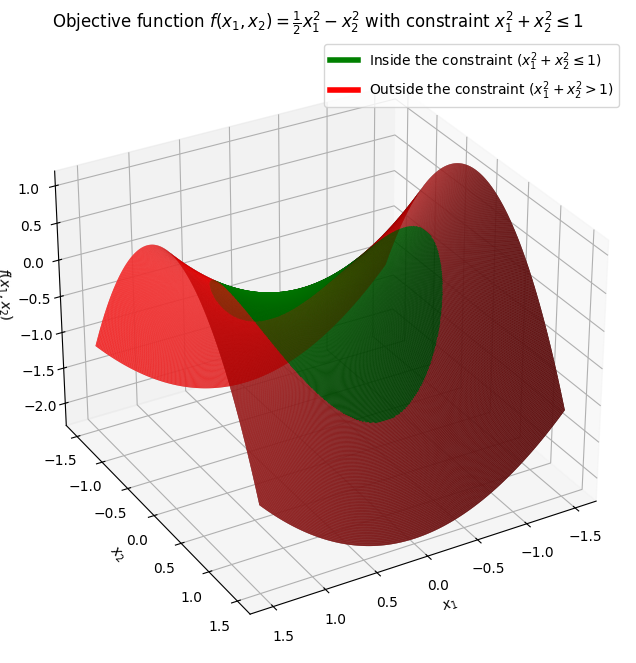
\includegraphics[width=1\textwidth]{A2.png}
    \caption{Constrained Optimization Problem}
    \label{A2}
\end{figure}
\begin{lstlisting}

import numpy as np
import matplotlib.pyplot as plt
from mpl_toolkits.mplot3d import Axes3D
from matplotlib.lines import Line2D

def f(x1, x2):
    return 0.5 * x1**2 - x2**2

x1 = np.linspace(-1.5, 1.5, 500)
x2 = np.linspace(-1.5, 1.5, 500)
X1, X2 = np.meshgrid(x1, x2)
Z = f(X1, X2)
mask = X1**2 + X2**2 <= 1

fig = plt.figure(figsize=(10, 8))
ax = fig.add_subplot(111, projection='3d')

surf_inside = ax.plot_surface(X1, X2, Z, rstride=1, cstride=1, facecolors=np.where(mask, 'g', 'lightgray'), edgecolor='none')

surf_outside = ax.plot_surface(X1, X2, Z, rstride=1, cstride=1, facecolors=np.where(mask, 'g', 'r'), edgecolor='none')

ax.set_xlabel('$x_1$')
ax.set_ylabel('$x_2$')
ax.set_zlabel('$f(x_1, x_2)$')

ax.set_title(r'Objective function $f(x_1, x_2) = \frac{1}{2}x_1^2 - x_2^2$ with constraint $x_1^2 + x_2^2 \leq 1$')

legend_elements = [Line2D([0], [0], color='g', lw=4, label='Inside the constraint ($x_1^2 + x_2^2 \leq 1$)'),
                   Line2D([0], [0], color='r', lw=4, label='Outside the constraint ($x_1^2 + x_2^2 > 1$)')]
ax.legend(handles=legend_elements, loc='upper right')
ax.view_init(elev=30, azim=60)  
plt.show()

\end{lstlisting}
\end{document}